\begin{figure}[!]
    \centering
    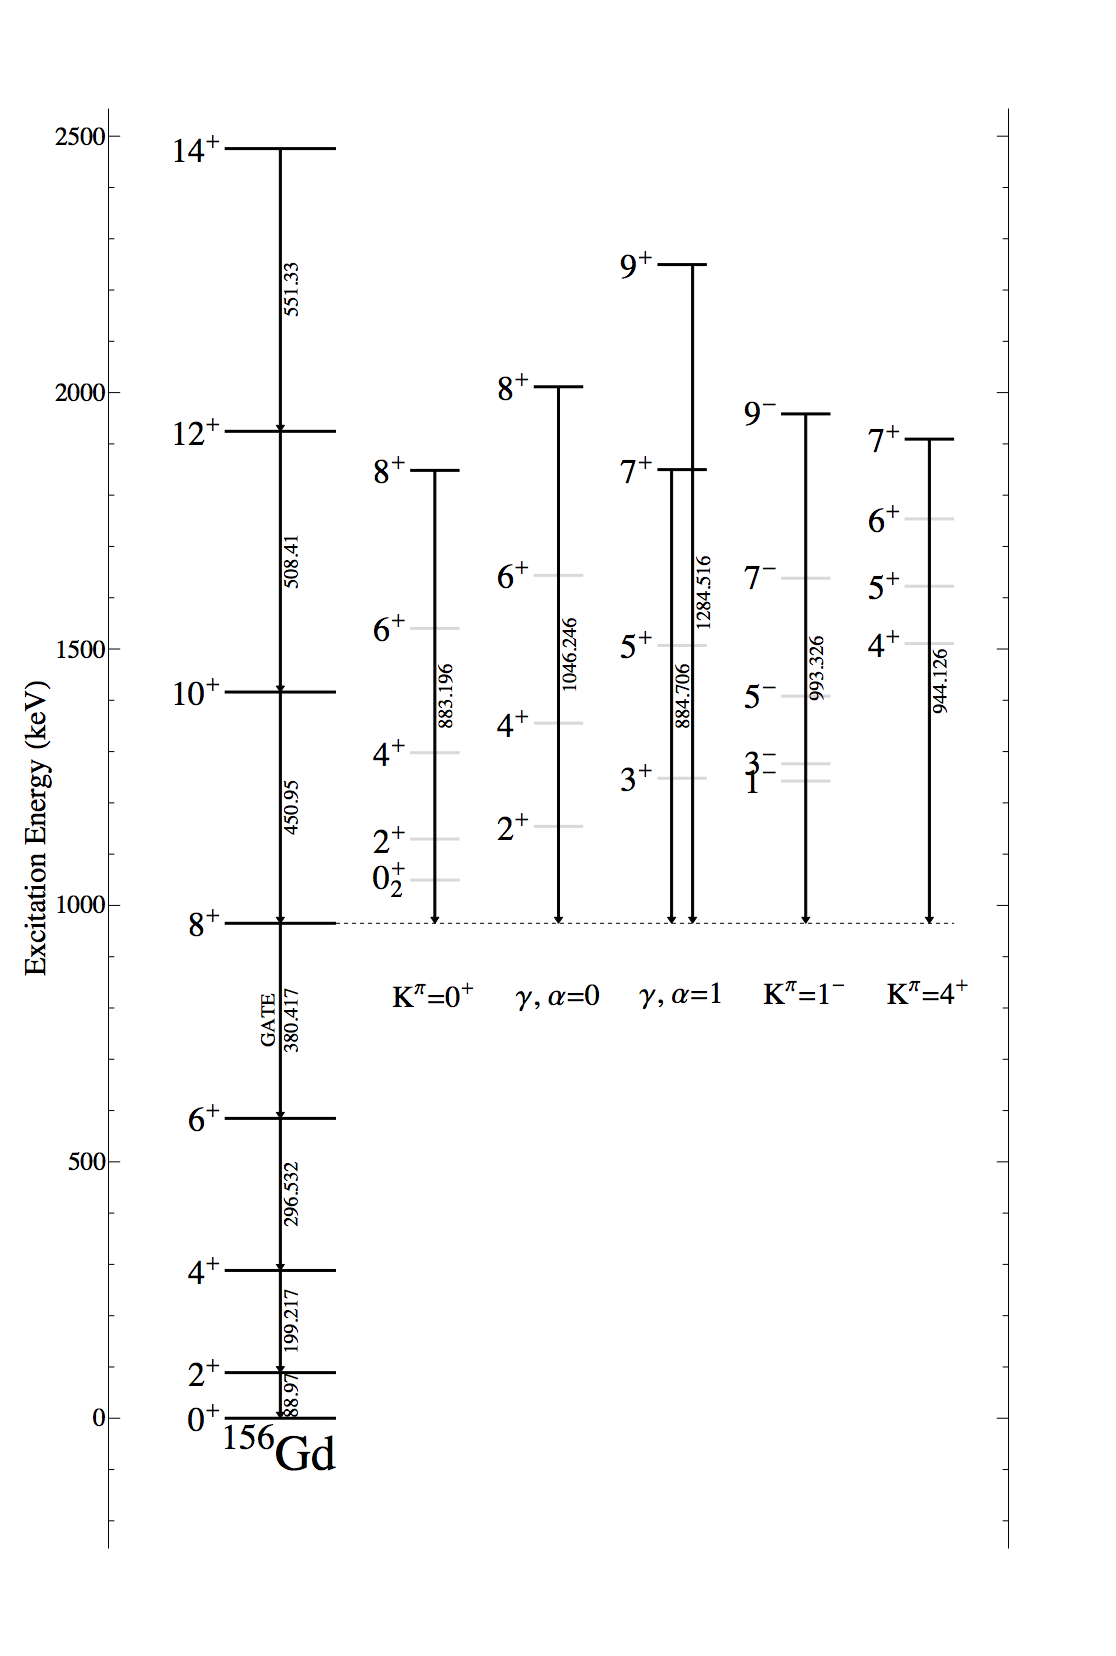
\includegraphics[scale=0.35]{156GdTablesAndFigs/156Gd_8to6.eps}
    \caption{Level Scheme of $^{156}$Gd. The gamma ray of the $8^+_{gs}\rightarrow 6^+_{gs}$ (380 keV) transition in the ground state was gated on. It was then compared with the gated spectrum from the gamma ray of the $10^+_{gs}\rightarrow 8^+_{gs}$ (451 keV) transition in the ground state. Peaks only appearing in the first gate were assumed to go into the $8^+_{gs}$ state, and assignments were made. Additionally, these peaks were also gated on, to look for cascades leading into the $8^+_{gs}$ state, which were found in several cases. The levels are organized by band. The lower levels of the band, unseen by gamma rays in this gate, are in blue.}
    \label{fig:156_8to6}
\end{figure}
\begin{figure}
    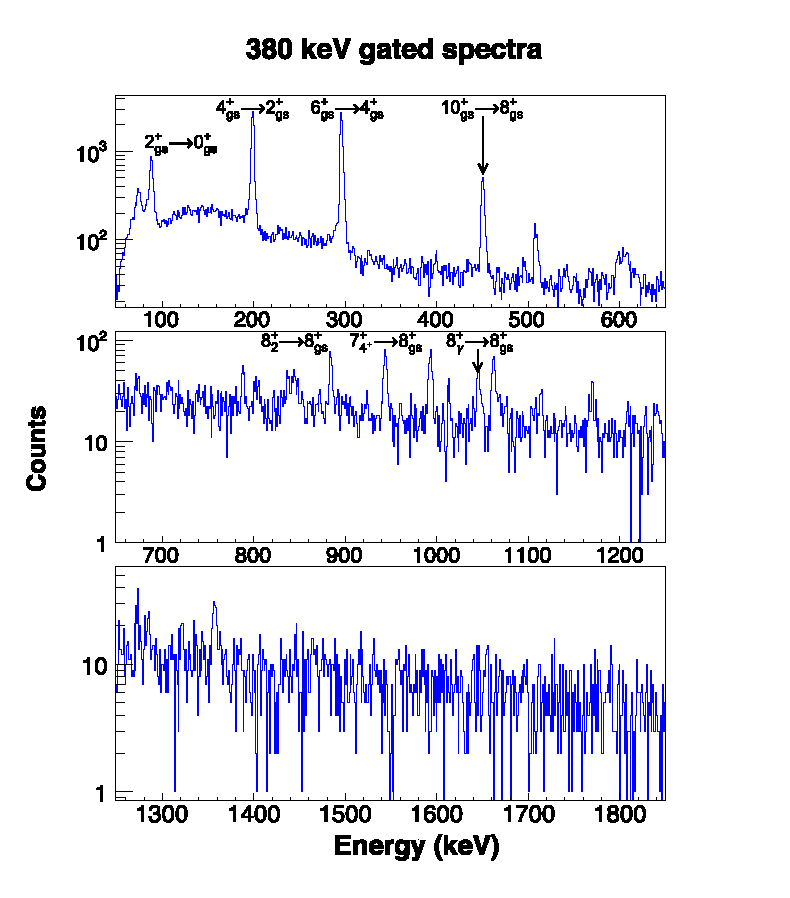
\includegraphics[scale=1.3]{156GdTablesAndFigs/380_gamma.eps}
    \caption{Gamma spectrum gated on 380 keV, corresponding to the $8^+_{gs}\rightarrow 6^+_{gs}$ transition. Several transitions are marked according to the level scheme in Figure \ref{fig:156_8to6}.}
    \label{fig:156_8to6spec}
\end{figure}